\documentclass[border=4pt]{standalone}
% Preámbulo común de las figuras. Cada figura es un documento standalone
% que se compila a SVG con scripts/build_figures.sh
\usepackage[utf8]{inputenc}
\usepackage{amsmath}
\usepackage{tikz}
\usepackage[american, siunitx]{circuitikz}
\usetikzlibrary{arrows.meta,calc,decorations.pathmorphing,patterns}
\tikzset{
  >={Stealth[length=2.2mm]},
  eje/.style={->, thin},
  hilo/.style={thick},
}
% Paleta común: tonos medios legibles sobre fondo claro
\definecolor{azul}{RGB}{31,94,168}
\definecolor{rojo}{RGB}{192,57,43}
\definecolor{verde}{RGB}{39,128,73}
\definecolor{naranja}{RGB}{211,120,30}
\definecolor{morado}{RGB}{125,60,152}

\begin{document}
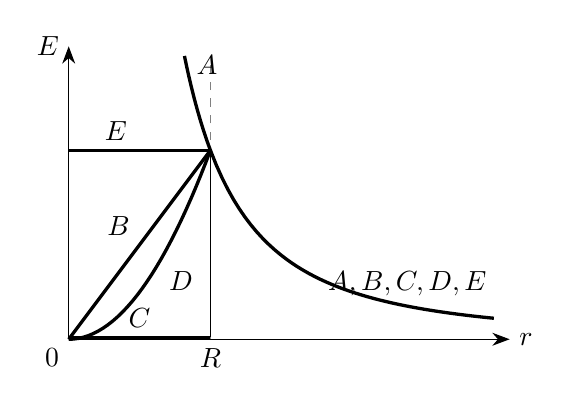
\begin{tikzpicture}[x=1.0cm, y=2.4cm]
  \draw[eje] (0,0) -- (5.6,0) node[right]{$r$};
  \draw[eje] (0,0) -- (0,1.55) node[left]{$E$};
  \node[below left] at (0,0) {$0$};
  \draw[dashed, gray] (1.8,0) node[below, black]{$R$} -- (1.8,1.5);
  % fuera de la esfera: todas iguales
  \draw[very thick] plot[domain=1.8:5.4, samples=50] (\x, {(1.8/\x)^2});
  \node[above] at (4.3,{(1.8/4.3)^2}) {$A,B,C,D,E$};
  % A: 1/r^2 en todas partes
  \draw[very thick] plot[domain=1.47:1.8, samples=30] (\x, {(1.8/\x)^2});
  \node[right] at (1.5,1.45) {$A$};
  % B: lineal
  \draw[very thick] (0,0) -- (1.8,1);
  \node[above left] at (0.9,0.5) {$B$};
  % C: cero dentro
  \draw[very thick] (0,0.01) -- (1.8,0.01);
  \draw[thin] (1.8,0.01) -- (1.8,1);
  \node[above] at (0.9,0.01) {$C$};
  % D: r^2
  \draw[very thick] plot[domain=0:1.8, samples=30] (\x, {(\x/1.8)^2});
  \node[below right] at (1.15,{(1.15/1.8)^2}) {$D$};
  % E: constante
  \draw[very thick] (0,1) -- (1.8,1);
  \node[above] at (0.6,1) {$E$};
\end{tikzpicture}
\end{document}
